\documentclass[fontset=windows, chinese, 10pt, xcolor=dvipsnames]{beamer}

\usepackage{amsmath,amssymb,mathtools}
\usepackage{xeCJK}
\usepackage{zhnumber}
\usepackage{tikz}
\usetikzlibrary{quotes,angles,arrows.meta,calc}

\usetheme{metropolis}
\usepackage{beamercolorthemeHistNanjing}

\newcommand{\red}[1]{\textcolor{red}{#1}}
\newcommand{\blue}[1]{\textcolor{blue}{#1}}
\newcommand{\green}[1]{\textcolor{green}{#1}}
\newcommand{\gray}[1]{\textcolor{gray}{#1}}
\newcommand{\orange}[1]{\textcolor{orange}{#1}}

\newcommand{\covfig}[1]{%
  \IfFileExists{tikz/#1.tex}%
    {\input{tikz/#1.tex}}%
    {\input{../../lecture_new/chapters/cov/figures/#1}}}

\newcommand{\sssub}[1]{ {\mathrm{#1} }}  % script size subscript\\\
\newcommand{\funcd}[2]{ \frac{d{#1}}{d{#2}}} %function full derivative
\newcommand{\funcpd}[2]{ \frac{\partial{#1}}{\partial{#2}}} %function partial derivative
\newcommand{\fnald}[2] { \frac{\delta {#1}}{\delta {#2}}} % functional derivative

\renewcommand{\Re}{\operatorname{Re}}
\renewcommand{\Im}{\operatorname{Im}}
\def\ext{\sssub{ext}}
\def\x{\sssub{x}}
\def\xc{\sssub{xc}}
\def\H{\sssub{H}}
\def\Hx{\sssub{Hx}}
\def\Hxc{\sssub{Hxc}}
\def\c{\sssub{c}}
\def\s{\sssub{s}}

% \def\ext{\sssub{ext}}
% \def\ext{\sssub{ext}}
% \def\ext{\sssub{ext}}
% \def\ext{\sssub{ext}}
% \defsssub{ext}


% definitions of bold faced symbols
\def\brpppp{{\mathbf{r}^{\prime\prime\prime\prime}}}
\def\brppp{{\mathbf{r}^{\prime\prime\prime}}}
\def\brpp{{\mathbf{r}^{\prime\prime}}}
\def\brp{{\mathbf{r}^{\prime}}}
\def\bzp{{\mathbf{z}^{\prime}}}
\def\bxp{{\mathbf{x}^{\prime}}}
\def\tp{{{t}^{\prime}}}
\def\tpp{{{t}^{\prime\prime}}}
\def\tppp{{{t}^{\prime\prime\prime}}}

\def\tbr{{\tilde{\mathbf{r}}}}
\def\bk{{\mathbf{k}}}
\def\br{{\mathbf{r}}}
\def\bp{{\mathbf{p}}}
\def\bq{{\mathbf{q}}}
\def\bv{{\mathbf{v}}}
\def\bz{{\mathbf{z}}}
\def\mbf{{\mathbf{f}}}

\def\bx{{\mathbf{x}}}
\def\bR{{\mathbf{R}}}
\def\bM{{\mathbf{M}}}
\def\bP{{\mathbf{P}}}
\def\bT{{\mathbf{T}}}
\def\bK{{\mathbf{K}}}
\def\bA{{\mathbf{A}}}
\def\bB{{\mathbf{B}}}
\def\bD{{\mathbf{D}}}
\def\bE{{\mathbf{E}}}
\def\bF{{\mathbf{F}}}
\def\bG{{\mathbf{G}}}
\def\bH{{\mathbf{H}}}
\def\bI{{\mathbf{I}}}
\def\bJ{{\mathbf{J}}}
\def\bP{{\mathbf{P}}}
\def\bS{{\mathbf{S}}}
\def\bV{{\mathbf{V}}}
\def\bX{{\mathbf{X}}}
\def\bY{{\mathbf{Y}}}
\def\dd{{\mathop{}\!\mathrm{d}}}
\def\dr{{\!\!\dd\br\,}}
\def\dx{{\!\!\dd\bx\,}}
\def\dy{{\!\!\dd\by\,}}
\def\dk{{\!\!\dd\bk\,}}
\def\dG{{\!\!\dd\bG\,}}


\def\half{{\frac{1}{2}}}
\def\tr{{\mathrm{tr}}}


\def\Arg{{\mathrm{Arg}\;}}
\def\arg{{\mathrm{arg}\;}}
\def\Res{{\mathrm{Res}\;}}


\title{变分法}
\subtitle{第一讲：泛函极值与 Euler–Lagrange 方程}

\date{\zhdigits{\the\year},\zhganzhinian{\the\year}年秋}
\author{罗凯}
\institute{南京理工大学物理学院}

\usebackgroundtemplate{%
\begin{tikzpicture}[remember picture,overlay]
  \node[opacity=0.05, at=(current page.center)] {
    
\includegraphics[width=0.6\paperwidth]{njust-logo.jpeg}
  };
\end{tikzpicture}}
\begin{document}

\begin{frame}
  \titlepage
\end{frame}

\AtBeginSubsection{
  \begin{frame}{提纲}
    \tableofcontents[currentsection,currentsubsection]
  \end{frame}
}

\begin{frame}{本章要抓住的那根纲}
  \begin{quote}
    变则通，通则久。\\
    \hfill ——《周易·系辞下》
  \end{quote}
  泛函极值把``求导''曲线从极值问题延伸到整条路径或整片场：
  \begin{itemize}
    \item 最短路径、最速降线、等周问题；
    \item Hamilton 原理、Lagrange 乘子法；
    \item 约束变分、密度泛函理论（DFT）。
  \end{itemize}
  本章贯穿这几条线索。
\end{frame}

\begin{frame}{本章提纲}
  \begin{enumerate}
    \item 泛函与 Euler–Lagrange 方程；
    \item Hamilton 原理与 Hamiltonian 力学；
    \item Lagrange 乘子法（含驻相与群速度、最大熵分布等物理实例）；
    \item 积分约束下的变分问题（最短弧、悬链线等）。
  \end{enumerate}
\end{frame}

% =============================================================
\section{泛函与 Euler–Lagrange 方程}

\subsection{什么是泛函}

\begin{frame}{函数与泛函}
  \begin{block}{函数}
    函数把数映射到数：$f:\mathbb{R}\to\mathbb{R}$，自变量是一个点。
  \end{block}
  \begin{block}{泛函}
    泛函把整条函数映射到数：$J:C[a,b]\to\mathbb{R}$，
    自变量是整条曲线、轨迹或场。方括号强调``整个函数''做论据。
  \end{block}
  普通优化里未知数是 $(x,y)$，变分问题里未知数是整条曲线 $y=u(x)$。
\end{frame}

\begin{frame}{最短路径作为泛函}
  固定端点 $u(a)=y_1$，$u(b)=y_2$ 的曲线长度为
  \begin{equation*}
    J[u]=\int_a^b\sqrt{1+u'(x)^2}\,\mathrm{d}x.
  \end{equation*}
  ``最短路径''即求使 $J[u]$ 取极小的容许函数 $u$。
  容许意味着函数具有所需的正则性且满足端点条件：曲线形状对，但端点错，就不在候选集里。
  \vspace{0.3em}
  同类例子还包括最速降线（捷线）时间、力学作用量、悬挂链条的势能。
\end{frame}

\begin{frame}{变分法的引子图}
  \begin{columns}[c]
    \begin{column}{0.50\textwidth}
      红线是候选曲线 $u(x)$，蓝虚线是变分后曲线 $u(x)+\varepsilon\eta(x)$。
      端点固定，$\eta(a)=\eta(b)=0$。
      当红色与蓝色曲线``几乎一致''时，泛函 $J[u]$ 的第一阶变化给出 Euler–Lagrange 方程。
    \end{column}
    \begin{column}{0.46\textwidth}
      \centering
      \scalebox{0.62}{\covfig{variation}}
    \end{column}
  \end{columns}
\end{frame}

\begin{frame}{拉格朗日密度}
  更一般的局域泛函写成
  \begin{equation*}
    J[u]=\int_a^b L\bigl(x,u,u'\bigr)\,\mathrm{d}x.
  \end{equation*}
  $L$ 称为\textbf{拉格朗日密度}：$L\,\mathrm{d}x$ 是小区间的贡献，积分把整条路径合在一起。
  高阶情形同样适用：
  \begin{equation*}
    J[u]=\int_a^b L\bigl(x,u,u',u'',\ldots\bigr)\,\mathrm{d}x.
  \end{equation*}
  局域意味着在 $x$ 处只依赖 $u$ 及该点的有限阶导数。
\end{frame}

\begin{frame}{容许变分}
  容许变分是单参数族
  \begin{equation*}
    u_\epsilon(x)=u(x)+\epsilon\eta(x),\qquad \eta(a)=\eta(b)=0.
  \end{equation*}
  $\eta$ 标明函数空间中变分方向，$\epsilon$ 标明走了多远。
  固定端点迫使 $\eta$ 在端点为零，否则变分后的曲线不再满足端点条件。
  \begin{itemize}
    \item 局域泛函 $J[u]=\int L\,\mathrm{d}x$ 通过 Euler–Lagrange 方程决定极值。
    \item 非局域泛函如 $J[u]=\frac12\iint u(x)K(x,x')u(x')\,\mathrm{d}x\,\mathrm{d}x'$，
      其导数含积分核。
  \end{itemize}
\end{frame}

\subsection{Euler–Lagrange 方程的推导}

\begin{frame}{泛函导数的定义}
  极值的第一阶条件是
  \begin{equation*}
    \delta J
    =\left.\frac{\mathrm{d}}{\mathrm{d}\epsilon}
      J[u+\epsilon\eta]\right|_{\epsilon=0}
    =0.
  \end{equation*}
  把被积函数展开到一阶：
  \begin{equation*}
    \delta J=\int_a^b
    \left(\frac{\partial L}{\partial u}\,\eta
     +\frac{\partial L}{\partial u'}\,\eta'
    \right)\mathrm{d}x.
  \end{equation*}
  这里 $L$ 在 $u+\epsilon\eta$ 处求值并保留一阶项。
\end{frame}

\begin{frame}{分部积分消去 $\eta'$}
  对第二项分部积分：
  \begin{equation*}
    \int_a^b\frac{\partial L}{\partial u'}\eta'\,\mathrm{d}x
    =\left[\frac{\partial L}{\partial u'}\eta\right]_a^b
    -\int_a^b\frac{\mathrm{d}}{\mathrm{d}x}
      \left(\frac{\partial L}{\partial u'}\right)\eta\,\mathrm{d}x.
  \end{equation*}
  固定端点意味着 $\eta(a)=\eta(b)=0$，边界项消失。
  剩下的被积函数里只有 $\eta$，任意性给出
  \begin{equation*}
    \boxed{\frac{\partial L}{\partial u}
    -\frac{\mathrm{d}}{\mathrm{d}x}
      \left(\frac{\partial L}{\partial u'}\right)=0.}
  \end{equation*}
  这就是 \textbf{Euler–Lagrange 方程}。
\end{frame}

\begin{frame}{变分法基本引理：系数逐点为零}
  如果对所有足够光滑且内部自由的扰动 $\eta$ 都有
  \begin{equation*}
    \int_a^b \Phi(x)\,\eta(x)\,\mathrm{d}x=0,
  \end{equation*}
  则 $\Phi(x)=0$ 在 $[a,b]$ 上逐点成立。
  把 $\eta$ 取为只在某小段上非零（即\textbf{检验函数}）就足够证明 $\Phi$ 在每一点都为零。
  这就是变分法能给出\textbf{逐点}微分方程的依据。
\end{frame}

\begin{frame}{例：最短路径是直线}
  最短路径
  \begin{equation*}
    L=\sqrt{1+u'^2},\qquad
    \frac{\partial L}{\partial u}=0.
  \end{equation*}
  Euler–Lagrange 方程化为
  \begin{equation*}
    \frac{\mathrm{d}}{\mathrm{d}x}
      \left(\frac{u'}{\sqrt{1+u'^2}}\right)=0,
  \end{equation*}
  即
  \begin{equation*}
    \frac{u'}{\sqrt{1+u'^2}}=\text{常量},\qquad
    u''=0.
  \end{equation*}
  极值曲线是直线，与``两点之间线段最短''一致。
  \vspace{0.3em}
  \centering
  \scalebox{0.62}{\covfig{straight_line}}
\end{frame}

\begin{frame}{例：最速降线不是直线}
  质点从静止沿曲线 $y=u(x)$ 在重力下无摩擦下滑。
  在高度 $u$ 处由能量守恒给出速率
  \begin{equation*}
    v=\sqrt{2g(y_0-u)}.
  \end{equation*}
  \begin{equation*}
    \mathrm{d}s=\sqrt{1+u'^2}\,\mathrm{d}x,\qquad
    \mathrm{d}t=\frac{\mathrm{d}s}{v},
  \end{equation*}
  滑落时间是泛函
  \begin{equation*}
    T[u]=\int_{x_0}^{x_1}
    \frac{\sqrt{1+u'^2}}
         {\sqrt{2g(y_0-u)}}\,\mathrm{d}x.
  \end{equation*}
  端点固定，求 $T$ 的极值，解是一条\textbf{摆线}（也称\textbf{捷线}）而非直线。
\end{frame}

\begin{frame}{最速降线图示}
  \begin{columns}[c]
    \begin{column}{0.42\textwidth}
      \centering
      \scalebox{0.55}{\covfig{cycloid}}
      \vspace{0.3em}
      {\small 红线为摆线（捷线，即最速降线），蓝虚线为同样端点下的直线（较慢）。}
    \end{column}
    \begin{column}{0.55\textwidth}
      \centering
      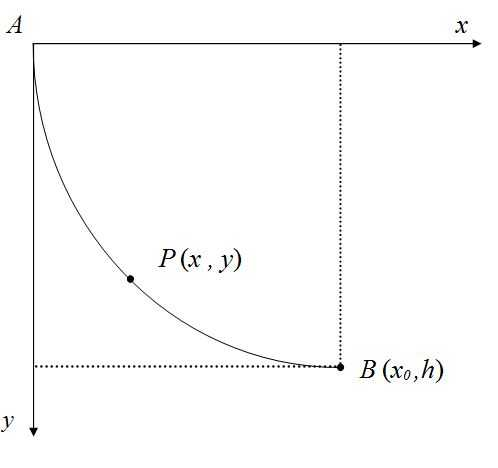
\includegraphics[width=0.95\textwidth]{figures/fastest_track.png}
    \end{column}
  \end{columns}
\end{frame}

\subsection{更一般的泛函导数}

\begin{frame}{高阶泛函与边界条件}
  允许导数阶为 $m$ 时，
  \begin{equation*}
    J[u]=\int_a^b
      L\bigl(x,u,u',u'',\ldots,u^{(m)}\bigr)\,\mathrm{d}x.
  \end{equation*}
  反复分部积分给出
  \begin{equation*}
    \frac{\delta J}{\delta u}
    =\sum_{k=0}^{m}(-1)^k\frac{\mathrm{d}^k}{\mathrm{d}x^k}
      \left(\frac{\partial L}{\partial u^{(k)}}\right).
  \end{equation*}
  $m=1$ 时即上节得到的形式（即标准的 Euler–Lagrange 方程）。
\end{frame}

\begin{frame}{自然边界条件}
  端点函数值固定时 $\eta(a)=\eta(b)=0$，边界项自动消失。
  若端点函数值不固定，则剩余边界项也必须为零，于是
  \begin{equation*}
    \left[\frac{\partial L}{\partial u'}\eta\right]_a^b=0.
  \end{equation*}
  对任意容许的 $\eta$ 成立，要求
  \begin{equation*}
    \left.\frac{\partial L}{\partial u'}\right|_a
    =\left.\frac{\partial L}{\partial u'}\right|_b=0.
  \end{equation*}
  这是端点函数值自由时变分原理``多产生''的方程，称为\textbf{自然边界条件}。
\end{frame}

\begin{frame}{场论的形式}
  对 $\mathbf{x}\in\Omega$ 上的场 $u(\mathbf{x})$，
  \begin{equation*}
    J[u]=\int_\Omega F(\mathbf{x},u,\partial_i u)\,\mathrm{d}^d\mathbf{x},
  \end{equation*}
  变分得
  \begin{equation*}
    \frac{\delta J}{\delta u}
    =\frac{\partial F}{\partial u}
    -\partial_i\!\left(\frac{\partial F}{\partial(\partial_i u)}\right).
  \end{equation*}
  形式与一维情形相同：把一维导数换成空间导数 $\partial_i$。
  这就是连续介质力学、静电学、波场理论与场论的统一表达。
\end{frame}

\begin{frame}{非局域泛函}
  非局域泛函耦合不同点的函数值。例如
  \begin{equation*}
    J[u]=\frac12\iint
    u(x)K(x,x')u(x')\,\mathrm{d}x\,\mathrm{d}x'.
  \end{equation*}
  当 $K$ 对称时，
  \begin{equation*}
    \frac{\delta J}{\delta u(x)}
    =\int K(x,x')u(x')\,\mathrm{d}x'.
  \end{equation*}
  非对称情形下写成 $\frac12\int[K(x,x')+K(x',x)]u(x')\,\mathrm{d}x'$。
  这正是 Hartree 项的形式，将在 DFT 部分再次出现。
\end{frame}

\subsection{多个因变量与场}

\begin{frame}{多个因变量}
  对 $u_1(x),\dots,u_n(x)$ 各自变分独立，Euler–Lagrange 方程为
  \begin{equation*}
    \frac{\partial L}{\partial u_i}
    -\frac{\mathrm{d}}{\mathrm{d}x}
        \left(\frac{\partial L}{\partial u_i'}\right)=0,
    \qquad i=1,\dots,n.
  \end{equation*}
  即使它们由同一拉格朗日密度耦合，每个分量仍然给出自己的方程。
\end{frame}

\begin{frame}{二维场：极小曲面方程}
  对 $u(x,y)$ 与
  \begin{equation*}
    J[u]=\iint_R
    F(x,y,u,u_x,u_y)\,\mathrm{d}x\,\mathrm{d}y,
  \end{equation*}
  场方程为
  \begin{equation*}
    F_u-\frac{\partial F_{u_x}}{\partial x}
         -\frac{\partial F_{u_y}}{\partial y}=0.
  \end{equation*}
  对 $F=\sqrt{1+u_x^2+u_y^2}$（肥皂膜面积），方程化为
  \begin{equation*}
    \frac{\partial}{\partial x}
    \!\left(\frac{u_x}{\sqrt{1+u_x^2+u_y^2}}\right)
    +\frac{\partial}{\partial y}
    \!\left(\frac{u_y}{\sqrt{1+u_x^2+u_y^2}}\right)=0.
  \end{equation*}
  这是\textbf{极小曲面方程}，表达平均曲率为零。
\end{frame}

\begin{frame}{DFT 视角}
  密度泛函理论 (DFT) 把粒子密度 $n(\mathbf{r})$ 作为基本场。
  约束为粒子数守恒
  \begin{equation*}
    \int n(\mathbf{r})\,\mathrm{d}^3\mathbf{r}=N,
  \end{equation*}
  引入化学势的 Lagrange 乘子 $\mu$ 得到增广泛函
  \begin{equation*}
    \widetilde E[n]=E[n]-\mu\Bigl(\int n-N\Bigr).
  \end{equation*}
  平稳条件为
  \begin{equation*}
    \frac{\delta E}{\delta n(\mathbf{r})}=\mu.
  \end{equation*}
  $\mu$ 在平衡态是常数，物理意义正是化学势。
\end{frame}

\begin{frame}{Thomas–Fermi 型能量}
  模型能量为
  \begin{equation*}
    E[n]=C\int n^{5/3}\,\mathrm{d}^3\mathbf{r}
         +\int v_{\mathrm{ext}} n\,\mathrm{d}^3\mathbf{r}
         +E_H[n],
  \end{equation*}
  其中 Hartree 贡献
  \begin{equation*}
    E_H[n]=\frac12\iint
    \frac{n(\mathbf{r})n(\mathbf{r}')}
         {|\mathbf{r}-\mathbf{r}'|}
    \,\mathrm{d}^3\mathbf{r}\,\mathrm{d}^3\mathbf{r}'.
  \end{equation*}
  逐项求泛函导数得到
  \begin{equation*}
    \frac{5}{3}C n^{2/3}+v_{\mathrm{ext}}+v_H=\mu.
  \end{equation*}
  局域项与全局项的耦合清晰：每项给出自己的泛函导数。
\end{frame}

\subsection{小结}

\begin{frame}{第一节小结}
  \begin{itemize}
    \item 泛函的自变量是整条函数；方括号强调``整个函数''做论据。
    \item $J[u]=\int L\,\mathrm{d}x$ 在 $u$ 取极值时满足
      $\frac{\partial L}{\partial u}
       -\frac{\mathrm{d}}{\mathrm{d}x}\bigl(\frac{\partial L}{\partial u'}\bigr)=0$。
    \item 边界条件：固定端点让 $\eta$ 在端点为零；自由端点产生自然边界条件
      $\partial L/\partial u'=0$。
    \item 场形式：$\frac{\delta J}{\delta u}
       =\frac{\partial F}{\partial u}
        -\partial_i\!\bigl(\frac{\partial F}{\partial(\partial_i u)}\bigr)$。
    \item DFT 把``约束的变分''翻译成``乘子 + 极值条件''的常规做法。
  \end{itemize}
\end{frame}

% =============================================================
\section{Hamilton 原理与哈密顿力学}

\subsection{广义坐标与作用量}

\begin{frame}{从 Newton 到 Lagrange}
  Newton 方程常用直角坐标写出，但物理系统有时用角度、约束距离、集体坐标更自然。
  这些变量称为\textbf{广义坐标} $q_i(t)$，不必具有长度量纲。
  对广义速度 $\dot q_i$，\textbf{作用量}定义为
  \begin{equation*}
    S[q]=\int_{t_1}^{t_2}
      L(q_i,\dot q_i,t)\,\mathrm{d}t.
  \end{equation*}
  \textbf{Hamilton 原理}说：在 $t_1,t_2$ 端点配置相同的邻近路径中，物理路径使 $S$ 取极值：
  \begin{equation*}
    \delta S=0.
  \end{equation*}
\end{frame}

\begin{frame}{Hamilton 原理与 Euler–Lagrange 方程}
  作用量的 Euler–Lagrange 方程就是
  \begin{equation*}
    \frac{\mathrm{d}}{\mathrm{d}t}\frac{\partial L}{\partial\dot q_i}
    -\frac{\partial L}{\partial q_i}=0.
  \end{equation*}
  若 $L=\frac12 m\dot{\mathbf{r}}^{\,2}-V(\mathbf{r})$（动能减势能），就回到
  \begin{equation*}
    m\ddot{\mathbf{r}}=-\nabla V=\mathbf{F}.
  \end{equation*}
  这表明 Euler–Lagrange 方程是 Newton 第二定律的坐标无关改写。
\end{frame}

\begin{frame}{Legendre 变换：$L\to H$}
  把速度变量换成\textbf{广义（正则）动量}
  \begin{equation*}
    p_i=\frac{\partial L}{\partial\dot q_i}.
  \end{equation*}
  \textbf{哈密顿量}是
  \begin{equation*}
    H(q_i,p_i,t)=p_i\dot q_i-L.
  \end{equation*}
  当 $\partial L/\partial\dot q_i$ 可对 $\dot q_i$ 反解时，$H$ 是 $(q,p,t)$ 的函数，定义在\textbf{相空间}上。
  对含速度相关相互作用或曲线坐标，$p_i$ 与``机械动量''可以不同。
\end{frame}

\begin{frame}{Hamilton 方程}
  对 $H$ 取微分，比较 $\mathrm{d}q_i,\mathrm{d}p_i,\mathrm{d}t$ 的系数，得到
  \begin{equation*}
    \dot q_i=\frac{\partial H}{\partial p_i},\qquad
    \dot p_i=-\frac{\partial H}{\partial q_i},\qquad
    \frac{\partial H}{\partial t}=-\frac{\partial L}{\partial t}.
  \end{equation*}
  这两套一阶方程与 Euler–Lagrange 等价，但\textbf{坐标与动量对称}。
  若 $L$ 不显含时间，则 $H$ 守恒。对普通力学系统，$H$ 通常就是总能。
\end{frame}

\begin{frame}{例子：自由粒子}
  自由粒子的 $L=\frac12 m\dot q^2$。
  共轭动量 $p=m\dot q$，哈密顿量 $H=p^2/(2m)$。
  Hamilton 方程
  \begin{equation*}
    \dot q=\frac{p}{m},\qquad \dot p=0.
  \end{equation*}
  $p$ 守恒，$\dot q=p/m$ 是匀速运动，与直觉一致。
\end{frame}

\begin{frame}{例子：简谐振子}
  $L=\frac12 m\dot q^2-\frac12 kq^2$，于是
  \begin{equation*}
    p=m\dot q,\qquad
    H=\frac{p^2}{2m}+\frac12 kq^2.
  \end{equation*}
  Hamilton 方程给出
  \begin{equation*}
    \dot q=\frac{p}{m},\qquad \dot p=-kq,
  \end{equation*}
  合并即 $m\ddot q+kq=0$，是熟知的简谐振子。
  在这里 $H$ 就是总能。
\end{frame}

\begin{frame}{第二节小结}
  \begin{itemize}
    \item Hamilton 原理：物理路径使作用量在端点固定的邻近路径中取极值。
    \item Euler–Lagrange 方程是 Newton 第二定律的坐标无关改写。
    \item Legendre 变换 $(q,\dot q,t)\to(q,p,t)$ 把拉格朗日量换成哈密顿量。
    \item Hamilton 方程把坐标与动量写成一对对称的一阶方程。
    \item $L$ 不显含 $t$ 时 $H$ 守恒；普通系统里 $H$ 即总能。
  \end{itemize}
\end{frame}

% =============================================================
\section{Lagrange 乘子法}

\subsection{方法}

\begin{frame}{问题设定}
  设 $f(\mathbf{x})$ 为目标函数，$c_a(\mathbf{x})=0\;(a=1,\dots,k)$ 为独立约束。
  引入增广函数
  \begin{equation*}
    \mathcal{F}(\mathbf{x},\lambda_a)
    =f(\mathbf{x})-\lambda_a c_a(\mathbf{x}).
  \end{equation*}
  把 $\mathbf{x}$ 与乘子 $\lambda_a$ 都视为独立变量，平稳方程是
  \begin{equation*}
    \frac{\partial f}{\partial x_i}
    -\lambda_a\frac{\partial c_a}{\partial x_i}=0,\qquad
    c_a(\mathbf{x})=0.
  \end{equation*}
  对 $\lambda_a$ 求导正好重新得到约束 $c_a=0$。
  ``乘子法''把约束吸收进极值搜索，代价是把空间扩大 $k$ 维。
\end{frame}

\begin{frame}{几何含义}
  \begin{columns}[c]
    \begin{column}{0.48\textwidth}
      $\nabla f$ 给出 $f$ 上升最快的方向，对应 $f$ 等值面的法向。
      在约束曲面上容许的 $\mathrm{d}\mathbf{x}$ 必须满足
      $\nabla c_a\cdot\mathrm{d}\mathbf{x}=0$。
      因此 $\nabla f$ 必须与切空间正交，即
      \[
      \nabla f=\lambda_a\nabla c_a.
      \]
      几何上 $\nabla f$ 是 $\{\nabla c_a\}$ 张成法向空间中的唯一向量。
    \end{column}
    \begin{column}{0.48\textwidth}
      \centering
      \scalebox{0.62}{\covfig{lagrange_multipliers}}
    \end{column}
  \end{columns}
\end{frame}

\begin{frame}{例：到平面的最近点}
  求平面 $x+y+z=1$ 上到原点的最近点。
  \begin{equation*}
    f=x^2+y^2+z^2,\qquad c=x+y+z-1.
  \end{equation*}
  方程组为
  \begin{equation*}
    2x-\lambda=0,\quad
    2y-\lambda=0,\quad
    2z-\lambda=0,\quad
    x+y+z=1.
  \end{equation*}
  因而 $x=y=z=1/3$，最近点是 $(1/3,1/3,1/3)$。
\end{frame}

\begin{frame}{例：双曲线上的极值}
  求 $f=x+y$ 在双曲线 $xy=1$ 上的临界点。
  \begin{equation*}
    1-\lambda y=0,\quad 1-\lambda x=0,\quad xy=1.
  \end{equation*}
  前两式给出 $x=y$，再代入约束 $xy=1$ 得
  $(1,1)$ 与 $(-1,-1)$ 两个点。
  几何意义：$x+y$ 的等值线与双曲线相切的两个位置。
\end{frame}

\subsection{驻相原理与群速度}

\begin{frame}{波动与色散关系}
  平面波叠加表示
  \begin{equation*}
    u(x,t)=\frac{1}{2\pi}\iint
      e^{\mathrm{i}(kx-\omega t)}\,U(k,\omega)\,\mathrm{d}k\,\mathrm{d}\omega.
  \end{equation*}
  但只有满足色散关系 $D(k,\omega)=0$ 的 $(k,\omega)$ 才能在介质中传播。
  对固定频率 $\omega=\omega(k)$，
  \begin{equation*}
    u(x,t)=\frac{1}{\sqrt{2\pi}}\int
      e^{\mathrm{i}(kx-\omega(k)t)}\,U(k)\,\mathrm{d}k.
  \end{equation*}
\end{frame}

\begin{frame}{驻相原理}
  一般 $k$ 处的相位 $\phi(k)=kx-\omega(k)t$ 振荡剧烈，不同波数的贡献相消。
  积分主要来自相位平稳点 $\phi'(k)=0$ 处。
  这是带约束的变分问题：让 $\phi(k)$ 在色散关系 $D(k,\omega)=0$ 下取极值。
  Lagrange 乘子方程为
  \begin{equation*}
    x-\lambda\,\partial D/\partial k=0,\qquad
    -t-\lambda\,\partial D/\partial\omega=0.
  \end{equation*}
  消去 $\lambda$ 得
  \begin{equation*}
    \frac{x}{t}=\frac{\partial\omega}{\partial k}=v_g.
  \end{equation*}
  这就是\textbf{群速度}：波包的主要能量以 $\partial\omega/\partial k$ 移动。
\end{frame}

\begin{frame}{例：声波}
  声波的色散关系 $\omega^2=c^2 k^2$，于是
  \begin{equation*}
    v_g=\frac{\partial\omega}{\partial k}=c.
  \end{equation*}
  群速度与相速度相等：声波无色散，尖锐脉冲传播时保持形状不变。
\end{frame}

\begin{frame}{例：深水重力波}
  深水表面波的色散关系 $\omega^2=gk$，于是
  \begin{equation*}
    v_p=\frac{\omega}{k}=\sqrt{g/k},\qquad
    v_g=\frac{\partial\omega}{\partial k}=\frac12\sqrt{g/k}.
  \end{equation*}
  群速度是相速度的一半：单个波峰从波包前端跑出，又在尾部重新形成。
  这就是为什么深水风浪中波长接近的波峰会比整个波包跑得更快。
\end{frame}

\subsection{多约束与高维情形}

\begin{frame}{一般维数}
  同一构造在多约束与高维情形下自然延伸。
  设 $\mathbb{R}^n$ 中有 $k$ 个独立约束，乘子 $\lambda_a$ 标记 $\nabla f$ 在 $\{\nabla c_a\}$ 这组基下的分量。
  方程数为 $n+k$，未知数也为 $n+k$，解通常唯一。
\end{frame}

\begin{frame}{例：球面上的高度极值}
  在单位球 $x^2+y^2+z^2=1$ 上求 $f=z$ 的极值。
  乘子方程
  \begin{equation*}
    0-\lambda\cdot 2x=0,\quad
    0-\lambda\cdot 2y=0,\quad
    1-\lambda\cdot 2z=0,
  \end{equation*}
  以及 $x^2+y^2+z^2=1$。
  前两式给出 $x=y=0$，再由 $\lambda\neq 0$ 得 $z=\pm 1$。
  极值是南北两极 $(0,0,\pm 1)$。
\end{frame}

\begin{frame}{例：环面上的四个极值}
  对环面
  \begin{equation*}
    c=\bigl(x^2+y^2+z^2+R^2-\rho^2\bigr)^2
      -4R^2(y^2+z^2)=0,\quad 0<\rho<R,
  \end{equation*}
  求 $f=z$ 的极值。乘子方程给出 $x=y=0$，
  约束化为
  \begin{equation*}
    (z^2+R^2-\rho^2)^2=4R^2 z^2,\quad
    z^2+R^2-\rho^2=\pm 2Rz.
  \end{equation*}
  四个解是
  \begin{equation*}
    (0,0,-R-\rho),\ (0,0,-R+\rho),\ (0,0,R-\rho),\ (0,0,R+\rho),
  \end{equation*}
  依次为极小、两个鞍点、极大。
\end{frame}

\begin{frame}{例：圆上最大面积多边形}
  把 $N$ 个顶点放在单位圆上。面积
  \begin{equation*}
    A=\frac12\sum_{i=1}^N
      \bigl(x_{i}y_{i+1}-x_{i+1}y_{i}\bigr),
    \quad (x_{N+1},y_{N+1})\equiv(x_1,y_1).
  \end{equation*}
  约束 $c_i=x_i^2+y_i^2-1=0$。
  变分得
  \begin{equation*}
    y_{i+1}-y_{i-1}=2\lambda_i x_i,\quad
    x_{i-1}-x_{i+1}=2\lambda_i y_i.
  \end{equation*}
  消去 $\lambda_i$ 后
  \begin{equation*}
    x_ix_{i+1}+y_iy_{i+1}
    =x_{i-1}x_i+y_{i-1}y_i.
  \end{equation*}
  含义：每条边与原点张成的内积方向余弦相同；最大面积多边形是\textbf{正多边形}。
\end{frame}

\subsection{信息不足时的概率分布（最大熵）}

\begin{frame}{最大熵原理}
  已知部分均值 $\langle\mathcal{O}_a\rangle$ 与归一化条件，
  在这些约束下最大化 Shannon 熵
  \begin{equation*}
    S=-\sum_{i=1}^N p_i\ln p_i.
  \end{equation*}
  增广函数为
  \begin{equation*}
    \mathcal{F}=-\sum_i p_i\ln p_i
      -\lambda_0\!\Bigl(\sum_i p_i-1\Bigr)
      -\sum_a\lambda_a\!\Bigl(\sum_i p_i\mathcal{O}_a
        -\langle\mathcal{O}_a\rangle\Bigr).
  \end{equation*}
  对 $p_i$ 求导给出
  \begin{equation*}
    p_i=\frac{1}{Z}\exp\!\Bigl(-\sum_a\lambda_a\mathcal{O}_a(x_i)\Bigr),
    \qquad
    Z=\sum_i\exp\!\Bigl(-\sum_a\lambda_a\mathcal{O}_a(x_i)\Bigr).
  \end{equation*}
  $\lambda_0$ 强制归一化，$\lambda_a$ 锁定均值；$Z$ 是配分函数。
\end{frame}

\begin{frame}{正则（玻尔兹曼）分布}
  若只有平均能量 $\langle E\rangle$ 一个约束（外加归一化），
  \begin{equation*}
    p_i=\frac{\mathrm{e}^{-\beta E_i}}{Z},\qquad
    Z=\sum_i\mathrm{e}^{-\beta E_i}.
  \end{equation*}
  $\beta$ 由 $\langle E\rangle=-\partial\ln Z/\partial\beta$ 隐式确定。
  这正是平衡统计力学的 \textbf{玻尔兹曼（Boltzmann）分布}。
  若再加上粒子数守恒，会出现 $\beta\mu$ 项。
\end{frame}

\subsection{临界点分类}

\begin{frame}{约束 Morse 指标}
  极值类型由约束切空间上的限制 Hessian 矩阵决定。
  对 $\mathbb{R}^n$ 中一个约束 $c=0$，切空间为
  \begin{equation*}
    T=\bigl\{\mathbf{v}\in\mathbb{R}^n
            :\nabla c(\mathbf{x}^\star)\cdot\mathbf{v}=0\bigr\}.
  \end{equation*}
  限制 Hessian
  \begin{equation*}
    H^T_{ij}=\partial_i\partial_j f
            -\lambda\,\partial_i\partial_j c
  \end{equation*}
  在 $T$ 上的特征值符号（正、负、零的个数）给出约束 Morse 指标。
\end{frame}

\begin{frame}{例：球面的极点}
  在 $f=z$、$c=x^2+y^2+z^2-1$、极点 $(0,0,1)$ 处，
  未约束的 Hessian 矩阵为零，乘子 $\lambda=1/2$，于是
  \begin{equation*}
    H^T_{ij}
    =-\frac12\,\partial_i\partial_j c
    =-\operatorname{diag}(1,1)
    \end{equation*}
  在切平面 $T=\{(x,y,0)\}$ 上。
  两个负特征值 $\Rightarrow$ 北极是约束极大。
\end{frame}

\begin{frame}{Euler 示性数}
  参数微扰时临界点成对出现、消失：
  \begin{equation*}
    \chi=\#\text{极小}-\#\text{鞍点}+\#\text{极大}
  \end{equation*}
  是个拓扑不变量，称为\textbf{Euler 示性数}（Euler characteristic）。
  若临界点非退化（Morse 临界点），Morse 引理说 $f$ 在邻域内可化为
  \begin{equation*}
    \pm x_1^2\pm x_2^2\cdots\pm x_{n-1}^2.
  \end{equation*}
  $n-1$ 个符号决定局部形态；负号个数即 Morse 指标。
\end{frame}

\begin{frame}{第三节小结}
  \begin{itemize}
    \item 引入乘子 $\lambda_a$，把约束极值化为增广函数的普通极值。
    \item 几何含义：$\nabla f=\lambda_a\nabla c_a$，$\nabla f$ 落在约束法向空间里。
    \item 驻相与群速度把乘子法推广到``约束条件是色散关系''的变分问题。
    \item 最大熵原理自动推出玻尔兹曼分布等平衡分布。
    \item 约束 Morse 指标与 Euler 示性数是分类临界点的工具。
  \end{itemize}
\end{frame}

% =============================================================
\section{积分约束下的变分问题}

\subsection{方法}

\begin{frame}{带积分约束的极值}
  积分约束约束的是整个函数，而不是有限个坐标。
  例：要求
  \begin{equation*}
    \int_a^b u(x)\,\mathrm{d}x=A,
  \end{equation*}
  同时极值
  \begin{equation*}
    J[u]=\int_a^b L(x,u,u')\,\mathrm{d}x.
  \end{equation*}
  引入常数乘子 $\lambda$，定义
  \begin{equation*}
    \widetilde J[u]=\int_a^b
      \bigl(L(x,u,u')+\lambda u\bigr)\,\mathrm{d}x-\lambda A.
  \end{equation*}
  对 $\lambda$ 变分恢复约束，对 $u$ 变分确定形状。
\end{frame}

\begin{frame}{化为普通 Euler–Lagrange 方程}
  $\lambda A$ 是常数项，对 $u$ 变分无影响。$\widetilde J$ 的 Euler–Lagrange 方程为
  \begin{equation*}
    \frac{\partial L}{\partial u}+\lambda
    -\frac{\mathrm{d}}{\mathrm{d}x}
      \left(\frac{\partial L}{\partial u'}\right)=0.
  \end{equation*}
  也就是说，积分约束只在方程里多出一个常数源项，
  这与有限维 Lagrange 乘子法完全平行。
\end{frame}

\subsection{最短弧与等周问题}

\begin{frame}{例：给定面积的最短弧}
  在端点固定、$\int u\,\mathrm{d}x=A$ 之下取
  $L=\sqrt{1+u'^2}$。Euler–Lagrange 方程为
  \begin{equation*}
    \lambda-\frac{\mathrm{d}}{\mathrm{d}x}
      \left(\frac{u'}{\sqrt{1+u'^2}}\right)=0.
  \end{equation*}
  第一次积分为
  \begin{equation*}
    \frac{u'}{\sqrt{1+u'^2}}=\lambda x+c.
  \end{equation*}
  再积一次得到圆弧方程
  \begin{equation*}
    (\lambda x+c)^2+(\lambda u-d)^2=1.
  \end{equation*}
  \begin{figure}
    \centering
    \scalebox{0.6}{\covfig{circle_curve}}
    \caption{最短弧是圆弧：固定面积约束下两固定端点间的极值曲线。}
  \end{figure}
  端点条件与面积条件定参数。
  几何上：面积要求把``直线''换成``常曲率曲线''。
\end{frame}

\begin{frame}{例：悬链线}
  均匀链条线密度 $\rho$，势能
  \begin{equation*}
    U[u]=\rho g\int_{-L/2}^{L/2}
      u(x)\sqrt{1+u'(x)^2}\,\mathrm{d}x.
  \end{equation*}
  长度约束
  \begin{equation*}
    \int_{-L/2}^{L/2}\sqrt{1+u'(x)^2}\,\mathrm{d}x=\ell.
  \end{equation*}
  增广拉格朗日量：$(\rho g u+\lambda)\sqrt{1+u'^2}$。
  Euler–Lagrange 方程化为
  \begin{equation*}
    u(x)=a\cosh\!\left(\frac{x-x_c}{a}\right)+u_c,
  \end{equation*}
  即\textbf{悬链线}。
  \begin{figure}
    \centering
    \scalebox{0.6}{\covfig{catenary}}
    \caption{悬链线方程为双曲余弦函数。}
  \end{figure}
  悬链线平衡了重力与张力；在小范围内可近似为抛物线。
\end{frame}

\begin{frame}{物理中的悬链线例子}
  \begin{figure}
    \centering
    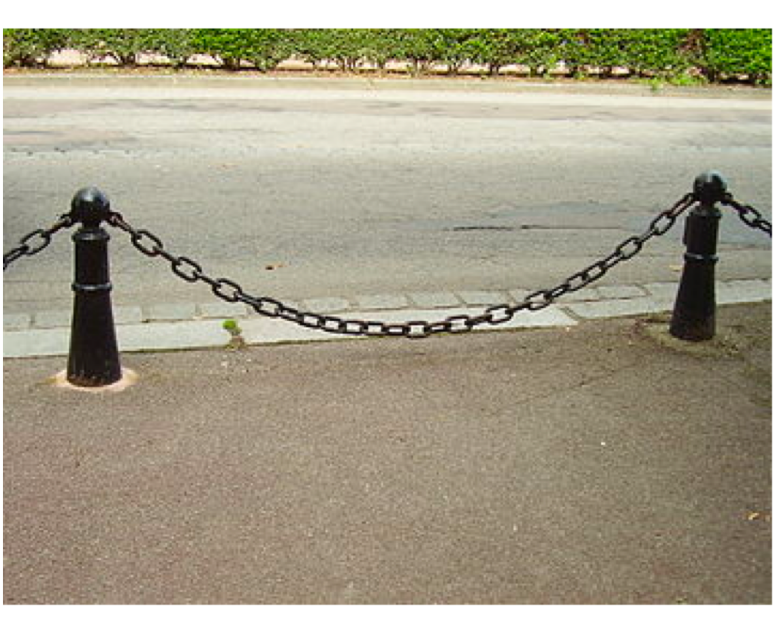
\includegraphics[width=0.42\textwidth]{figures/roadside.png}
    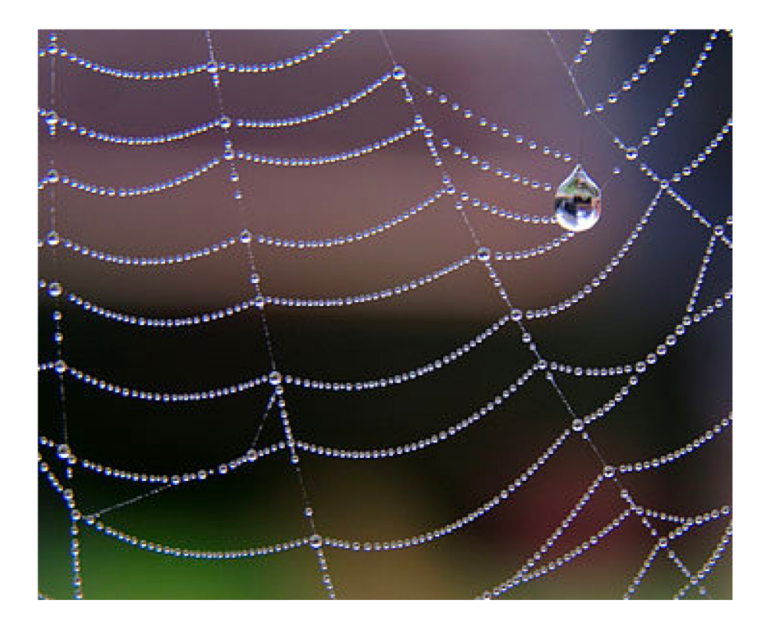
\includegraphics[width=0.42\textwidth]{figures/cobweb.png}
    \caption{悬链线状曲线的物理例子。}
  \end{figure}
\end{frame}

\begin{frame}{与有限维乘子的对照}
  积分约束下的乘子法是有限维 Lagrange 乘子法的函数空间类比：
  \begin{itemize}
    \item 对 $\lambda$ 变分恢复约束（$\delta\widetilde J/\delta\lambda=0$）；
    \item 对 $u$ 变分给出 Euler–Lagrange 方程。
  \end{itemize}
  这也是``归一化密度问题''里常数化学势 $\mu$ 的来源。
\end{frame}

\begin{frame}{本章小结}
  \begin{itemize}
    \item 泛函极值把``对一个数的导数''推广到``对整条函数的导数''。
    \item Euler–Lagrange 方程、Hamilton 原理、Lagrange 乘子法是三件套；
      它们互相支撑，又各自独立。
    \item 哈密顿量由 Legendre 变换给出，与 Euler–Lagrange 方程等价。
    \item 约束极值：有限维是乘子 $\lambda_a$，函数空间是``常数乘子 $\lambda$''。
    \item 物理例子：最速降线、悬链线、群速度、最大熵分布、DFT 平衡密度。
  \end{itemize}
\end{frame}

\begin{frame}{扩展阅读}
  \begin{itemize}
    \item Gelfand \& Fomin, \textit{Calculus of Variations}.
    \item Goldstein, \textit{Classical Mechanics}.
    \item Arfken, Weber \& Harris, \textit{Mathematical Methods for Physicists}.
    \item Byron \& Fuller, \textit{Mathematics of Classical and Quantum Physics}.
  \end{itemize}
\end{frame}

\end{document}